\documentclass[11pt]{article}
\usepackage{amsmath, amsfonts, amsthm, amssymb}  % Some math symbols
\usepackage{lmodern}  % A modern version of LaTeX's famous default font. 
\usepackage{microtype}
\usepackage{fullpage}

\usepackage[x11names, rgb]{xcolor}
\usepackage{graphicx}
\usepackage{tikz}
\usetikzlibrary{decorations,arrows,shapes,automata,positioning}
\tikzset{
->, % makes the edges directed
% >=stealth’, % makes the arrow heads bold
node distance=1cm, % specifies the minimum distance between two nodes. Change if necessary.
every state/.style={thick, fill=gray!10}, % sets the properties for each ’state’ node
initial text=$ $, % sets the text that appears on the start arrow
auto
}

\usepackage{etoolbox}
\usepackage{enumerate}
\usepackage{listings}
\usepackage{syntax}
\setlength{\parindent}{0pt}
\setlength{\parskip}{5pt plus 1pt}

\newcommand{\nopagenumbers}{
    \pagestyle{empty}
}

\def\indented#1{\list{}{}\item[]}
\let\indented=\endlist

\providetoggle{questionnumbers}
\settoggle{questionnumbers}{true}
\newcommand{\noquestionnumbers}{
    \settoggle{questionnumbers}{false}
}

\newcounter{questionCounter}
\newenvironment{question}[2][\arabic{questionCounter}]{%
    \addtocounter{questionCounter}{1}%
    \setcounter{partCounter}{0}%
    \vspace{.25in} \hrule \vspace{0.4em}%
        \noindent{\bf \iftoggle{questionnumbers}{#1: }{}#2}%
    \vspace{0.8em} \hrule \vspace{.10in}%
}{$ $\newpage}

\newcounter{partCounter}[questionCounter]
\renewenvironment{part}[1][\alph{partCounter}]{%
    \addtocounter{partCounter}{1}%
    \vspace{.10in}%
    \begin{indented}%
       {\bf (#1)} %
}{\end{indented}}

\def\show#1{\ifdefempty{#1}{}{#1\\}}




%%%%%%%%%%%%%%%%% Identifying Information %%%%%%%%%%%%%%%
%%		 		For 301, we'd rather you DIDN'T tell us who you are   		%%
%%				in your homework so that we're not biased when we     		%%
%% 				grade. So, even if you fill this information in, it   			%%
%% 				will not show up in the document unless you uncomment 		%%
%%				 \show\myname and \show\myemail below                  		%%
%%%%%%%%%%%%%%%%%%%%%%%%%%%%%%%%%%%%%%%%%%%
\newcommand{\myhwname}{Homework 3}
\newcommand{\myname}{ChessZra}
\newcommand{\myemail}{jsee4@uic.edu}
%%%%%%%%%%%%%%%%%%%%%%%%%%%%%%%%%%%%%%%%%%%%%%%%%%%%%%%%%%%
\newcommand{\header}{%
\begin{center}
    {\Large \show\myhwname}
    % \show\myname
    % \show\myemail
    \today
\end{center}}
%%%%%%%%%%%%%%%%%%% Document Options %%%%%%%%%%%%%%%%%%%%%%
% \noquestionnumbers
\nopagenumbers
%%%%%%%%%%%%%%%%%%%%%%%%%%%%%%%%%%%%%%%%%%%%%%%%%%%%%%%%%%%

\begin{document}
\header

\begin{question}{Regular Grammars}
    \begin{center}
        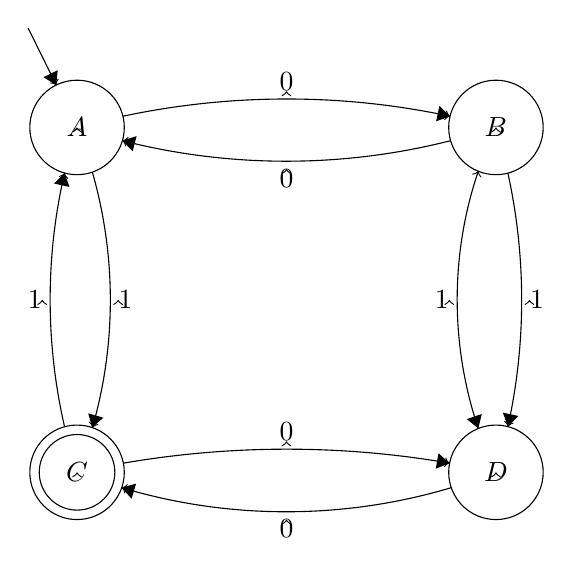
\begin{tikzpicture}[scale=0.2]
        \tikzstyle{every node}+=[inner sep=0pt]
        \draw [black] (24.9,-14.9) circle (3);
        \draw (24.9,-14.9) node {$A$};
        \draw [black] (51.5,-14.9) circle (3);
        \draw (51.5,-14.9) node {$B$};
        \draw [black] (24.9,-36.8) circle (3);
        \draw (24.9,-36.8) node {$C$};
        \draw [black] (24.9,-36.8) circle (2.4);
        \draw [black] (51.5,-36.8) circle (3);
        \draw (51.5,-36.8) node {$D$};
        \draw [black] (21.8,-8.6) -- (23.58,-12.21);
        \fill [black] (23.58,-12.21) -- (23.67,-11.27) -- (22.77,-11.71);
        \draw [black] (27.814,-14.188) arc (102.01221:77.98779:49.905);
        \fill [black] (48.59,-14.19) -- (47.91,-13.53) -- (47.7,-14.51);
        \draw (38.2,-12.6) node [above] {$0$};
        \draw [black] (48.621,-15.741) arc (-75.75521:-104.24479:42.35);
        \fill [black] (27.78,-15.74) -- (28.43,-16.42) -- (28.68,-15.45);
        \draw (38.2,-17.54) node [below] {$0$};
        \draw [black] (50.379,-34.019) arc (-161.39772:-198.60228:25.609);
        \fill [black] (50.38,-34.02) -- (50.6,-33.1) -- (49.65,-33.42);
        \draw (48.54,-25.85) node [left] {$1$};
        \draw [black] (52.259,-17.801) arc (12.3795:-12.3795:37.542);
        \fill [black] (52.26,-33.9) -- (52.92,-33.22) -- (51.94,-33.01);
        \draw (53.63,-25.85) node [right] {$1$};
        \draw [black] (27.843,-36.218) arc (99.78544:80.21456:60.94);
        \fill [black] (48.56,-36.22) -- (47.85,-35.59) -- (47.68,-36.57);
        \draw (38.2,-34.83) node [above] {$0$};
        \draw [black] (48.664,-37.775) arc (-73.38709:-106.61291:36.598);
        \fill [black] (27.74,-37.77) -- (28.36,-38.48) -- (28.65,-37.52);
        \draw (38.2,-39.8) node [below] {$0$};
        \draw [black] (24.107,-33.907) arc (-167.0655:-192.9345:35.997);
        \fill [black] (24.11,-17.79) -- (23.44,-18.46) -- (24.42,-18.68);
        \draw (22.69,-25.85) node [left] {$1$};
        \draw [black] (25.872,-17.737) arc (15.99782:-15.99782:29.438);
        \fill [black] (25.87,-33.96) -- (26.57,-33.33) -- (25.61,-33.06);
        \draw (27.51,-25.85) node [right] {$1$};
        \end{tikzpicture}
        \end{center}
\end{question}

\begin{question}{Context Is Everything (Except for CFGs)}
	\begin{part}
        \begin{align*}
            &S \rightarrow T \,|\, bSaaa \\
            &T \rightarrow \epsilon \,|\, aTaa
        \end{align*}
	\end{part}

	\begin{part}
        \begin{align*}
            &S \rightarrow A00B \\
            &B \rightarrow \epsilon \,|\, 0B \\
            &A \rightarrow \epsilon \,|\, 110A \,|\, 01A
        \end{align*}
	\end{part}

	\begin{part}
        \begin{align*}
            &S \rightarrow \epsilon \,|\, 01 \,|\, 10 \,|\, 0011 \,|\, 0101 \,|\, 0110 \,|\, 1001 \,|\, 1010 \,|\, 1100 \\
        \end{align*} 
	\end{part}
\end{question}

\begin{question}{Noam, Is This Normal?}
    \begin{align*}
        &S \rightarrow 0XY \,|\, Y \\
        &X \rightarrow 1X \,|\, Y \\
        &Y \rightarrow S \,|\, 0 \,|\, \epsilon \\
    \end{align*} 
    START:
    \begin{align*}
        &S_1 \rightarrow S\\
        &S \rightarrow 0XY \,|\, Y \\
        &X \rightarrow 1X \,|\, Y \\
        &Y \rightarrow S \,|\, 0 \,|\, \epsilon \\
    \end{align*} 
    BIN:
    \begin{align*}
        &S_1 \rightarrow S\\
        &S \rightarrow 0T \,|\, Y \\
        &X \rightarrow 1X \,|\, Y \\
        &Y \rightarrow S \,|\, 0 \,|\, \epsilon \\
        &T \rightarrow XY \\
    \end{align*} 
    DEL:
    \begin{align*}
        &S_1 \rightarrow S \,|\, \epsilon\\
        &S \rightarrow 0T \,|\, Y \,|\, 0 \\
        &X \rightarrow 1X \,|\, Y \,|\, 1 \\
        &Y \rightarrow S \,|\, 0 \\
        &T \rightarrow XY \,|\, X \,|\, Y \\
    \end{align*} 
    UNIT:
    \begin{align*}
        &S_1 \rightarrow 0T \,|\, 0 \,|\, \epsilon\\
        &S \rightarrow 0T \,|\, 0 \\
        &X \rightarrow 1X \,|\, 1 \,|\, 0 \,|\, 0T \\
        &Y \rightarrow 0 \,|\, 0T \\
        &T \rightarrow XY \,|\, 1X \,|\, 1 \,|\, 0 \,|\, 0T \\
    \end{align*} 
    TERM:
    \begin{align*}
        &S_1 \rightarrow BT \,|\, B \,|\, \epsilon\\
        &S \rightarrow BT \,|\, B \\
        &X \rightarrow AX \,|\, A \,|\, B \,|\, BT \\
        &Y \rightarrow B \,|\, BT \\
        &T \rightarrow XY \,|\, AX \,|\, A \,|\, B \,|\, BT \\
        &A \rightarrow 1 \\
        &B \rightarrow 0 \\
    \end{align*} 
\end{question}
\end{document}
